\documentclass[submit,techrep]{ipsj}

\usepackage[dvipdfmx]{graphicx}
\usepackage{latexsym}
\usepackage{url}
\usepackage{here}

\def\Underline{\setbox0\hbox\bgroup\let\\\endUnderline}
\def\endUnderline{\vphantom{y}\egroup\smash{\underline{\box0}}\\}
\def\|{\verb|}

\setcounter{巻数}{53}%vol53=2012
\setcounter{号数}{10}
\setcounter{page}{1}

% インタラクション特有の設定。印刷工程で柱・ノンブルの埋め込みを行う。
\makeatletter
\pagestyle{empty}
\def\@oddhead{}%
\def\@evenhead{}%
\def\ps@IPSJTITLEheadings{}
\makeatother

\long\def\comment#1{}

\begin{document}

\title{わかるらんど: IoT時代の情報共有視覚化}
\etitle{WakaruLand: An information visualization system for the IoT age}

\affiliate{MG}{慶應義塾大学大学院 政策・メディア研究科}
\affiliate{EI}{慶應義塾大学 環境情報学部}

\author{山田 尚昭}{Naoaki Yamada}{MG}
\author{増井 俊之}{Toshiyuki Masui}{EI}

\begin{abstract}
人や環境の状態がリアルタイムにわかる視覚化システム「わかるらんど」を提案する.
単一の画面にタイル状に情報を並べて表示するダッシュボードは複数のフロー情報をひと目でチェックするのに効果的な視覚化手法である.
しかし,人間の感情や現在の状況もフロー情報であるが,それらをアウトプットにはSNSが用いられダッシュボードに表示することは今まで行われてこなかった.
これはSNSに投稿される長いテキストメッセージはダッシュボードに表示するには適さないからである.
わかるらんどは人間の感情や現在の状況を,近年のメッセンジャーアプリで利用されているスタンプで表現することで,
ダッシュボードにリアルタイムに人間の感情や現在の状況を表示することを可能にした.
わかるらんどはありとあらゆる場所におけるサイネージや会議やコンファレンスでのチャットシステムとして極めて汎用的な利用が期待できる.
\end{abstract}

\maketitle

\section*{修正とか必要なところ}

\begin{itemize}
  \item わかるらんどの思想を述べる (section 2)
  \item 消去性コンピューティングについて\cite{kurihara2016}
  \item linda-serverじゃなくてWebLindaにすればどうか
\end{itemize}

\section{はじめに}

インターネット上の情報は利用する目的や形態から\textgt{フロー情報}と\textgt{ストック情報}の2つに分類できる.

\subsection*{フロー情報}

SNS,ニュース,IoT機器などリアルタイムに更新される情報.

\subsection*{ストック情報}

辞書,公式サイト,論文などいつでも参照できる情報.\vspace{0.2in}

現在のインターネットには特にフロー情報が溢れており,それらを情報の鮮度が落ちないうちに見ることができるインタフェースが求められている.

フロー情報を視覚化する手法として\textgt{ダッシュボード}(図\ref{dashing})がある.
ダッシュボードとは単一の画面に複数の情報をタイル状に並べて表示するもの\cite{few2005}で,センサの値や株価などのフロー情報をひと目で把握するのに非常に便利である.
ダッシュボードには様々な製品やサービスが存在し,多くの組織の壁掛けのディスプレイやデジタルサイネージで利用されている.
しかし,フロー情報のひとつである「人間の感情や現在の状況」というものをダッシュボードに表示することは行われてこなかった.
人間の感情や現在の状況をアウトプットする場としてSNSが利用されているが,数文字程度を表示するのが限度のダッシュボードのセルに表示するには適していない.
人間の感情や現在の状況をダッシュボードに表示するのに適した形でアウトプットできれば,タイムラインよりも遥かに効率良く,
大勢の人間の感情や現在の状況をひと目でチェックできるとのではないかと考えた.

本論文では,一般的にダッシュボードに表示される情報に加えて,人間の感情や現在の状況をスタンプで表現し表示することによって,
ありとあらゆるフロー情報を単一の画面に表示できる視覚化システム「\textgt{わかるらんど}」について述べる.

\begin{figure}[h]
\centering
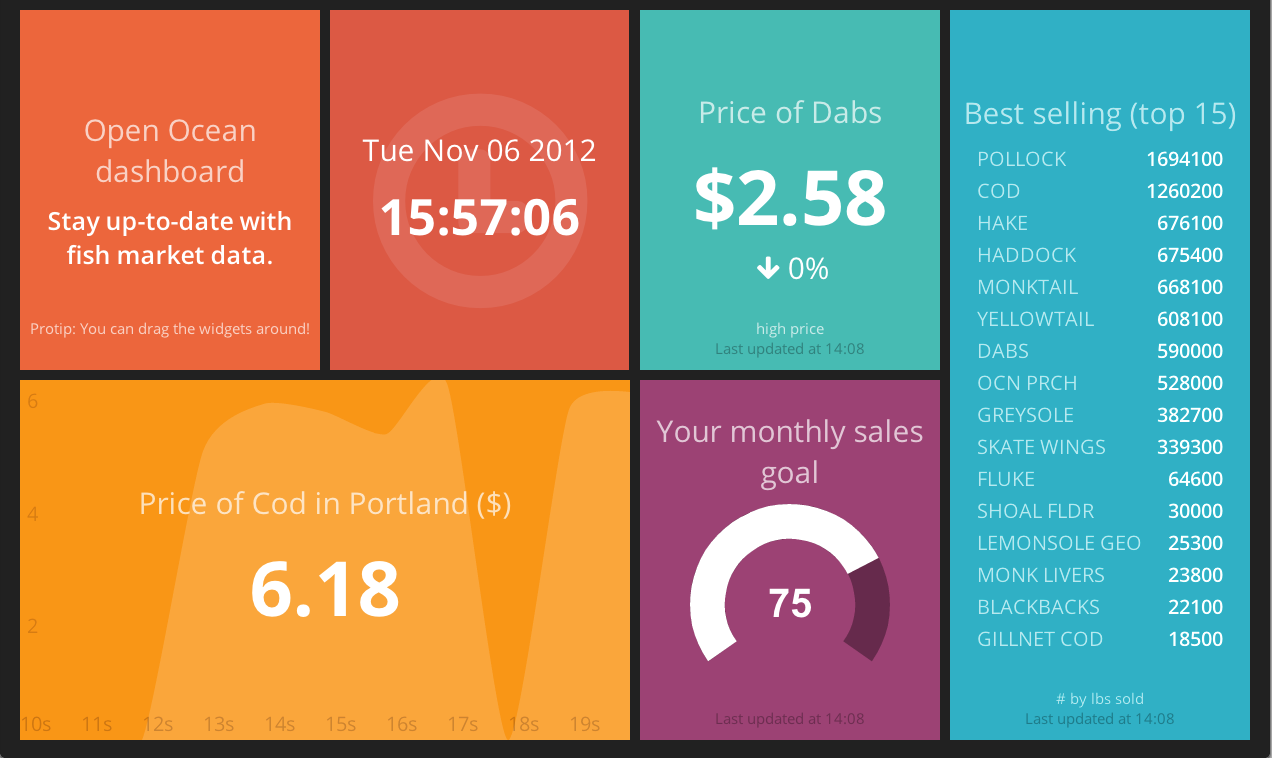
\includegraphics[width=7cm]{images/dashing.png}
\caption{Dashingによって作成されたダッシュボード}
\label{dashing}
\end{figure}
\section{わかるらんど}
本章では、我々の開発した『わかるらんど』の機能と使用方法について述べる。

\subsection{ユーザインタフェース}
『わかるらんど』のユーザインタフェースは「ダッシュボード」と「投稿画面」の2つからなる。
図\ref{dashboard}はダッシュボードのスクリーンショットである.
インフォメーションダッシュボードのようにセンサのデータを表示したり、
ユーザがリアクションとしてテキストやスタンプを投稿したものをリアルタイムに
1つの画面に表示することができる。
センサのデータなどは自動的に更新され、ユーザのリアクションは図\ref{console}の投稿画面で
ユーザ名を入力し、スタンプを一覧から選んで投稿することで自分のアイコンの上にオーバーレイ表示される。
リアクションの投稿には表示時間が設定されており、指定時間が経過すると自動的に投稿が取り下げられるため
いつまでも古い投稿が表示され続けてしまうということはない。
ダッシュボードと投稿画面は画面右上のボタンで切り替えることができる。
また、投稿するスタンプは投稿画面でユーザが自由に追加/削除することができる。

\begin{figure}[h]
\centering
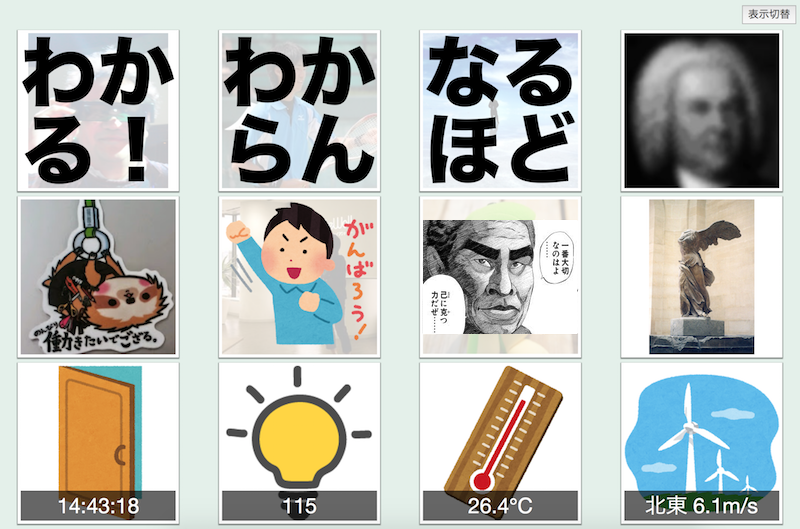
\includegraphics[width=7cm]{images/dashboard.png}
\caption{『わかるらんど』のダッシュボード}
\label{dashboard}
\end{figure}

\begin{figure}[h]
\centering
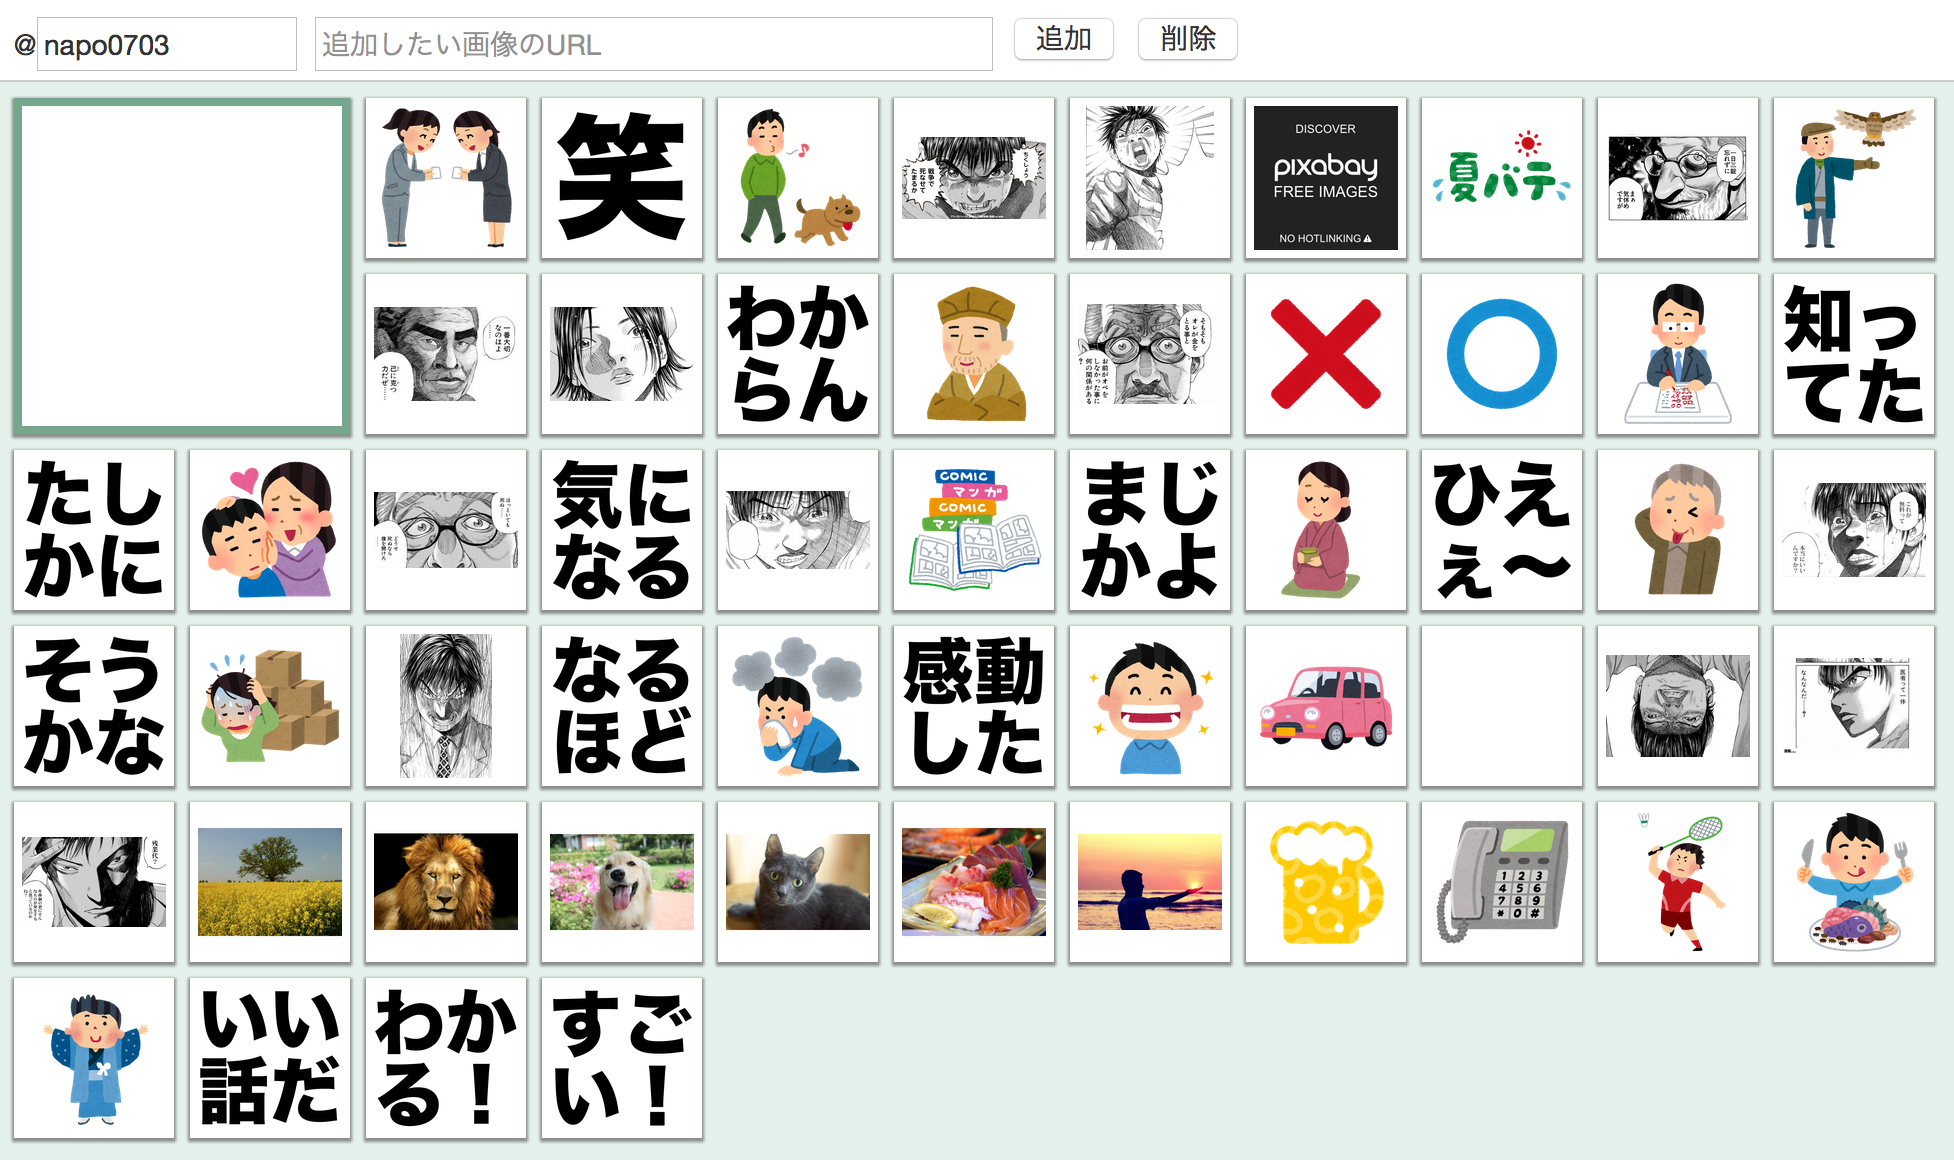
\includegraphics[width=7cm]{images/console.png}
\caption{『わかるらんど』の投稿画面}
\label{console}
\end{figure}

\subsection{表示するユーザとデータの指定}
『わかるらんど』のダッシュボードに表示されるセルは、ユーザのテキストや画像のスタンプを表示する
「リアクション」セルと、センサやWebの情報を表示する「データ」セルの2種類がある(図\ref{cell})。

\begin{figure}[h]
\centering

\includegraphics[width=7cm]{images/cell.png}
\caption{リアクション(左)とデータ(右)}
\label{cell}
\end{figure}

ダッシュボードに表示するユーザのリアクションの指定は、
\url{https://wakaruland.com/@napo0703,@masui,@shokai,@dorayaki0}
のようにURLの末尾にカンマ区切りでTwitterのユーザ名を「\url{@}」を付けて書くことで行う。
この場合は図\ref{n_m_s_d}のように\url{@napo0703,@masui,@shokai,@dorayaki0}の4人のユーザのセルが
ダッシュボードに表示される。

\begin{figure}[h]
\centering
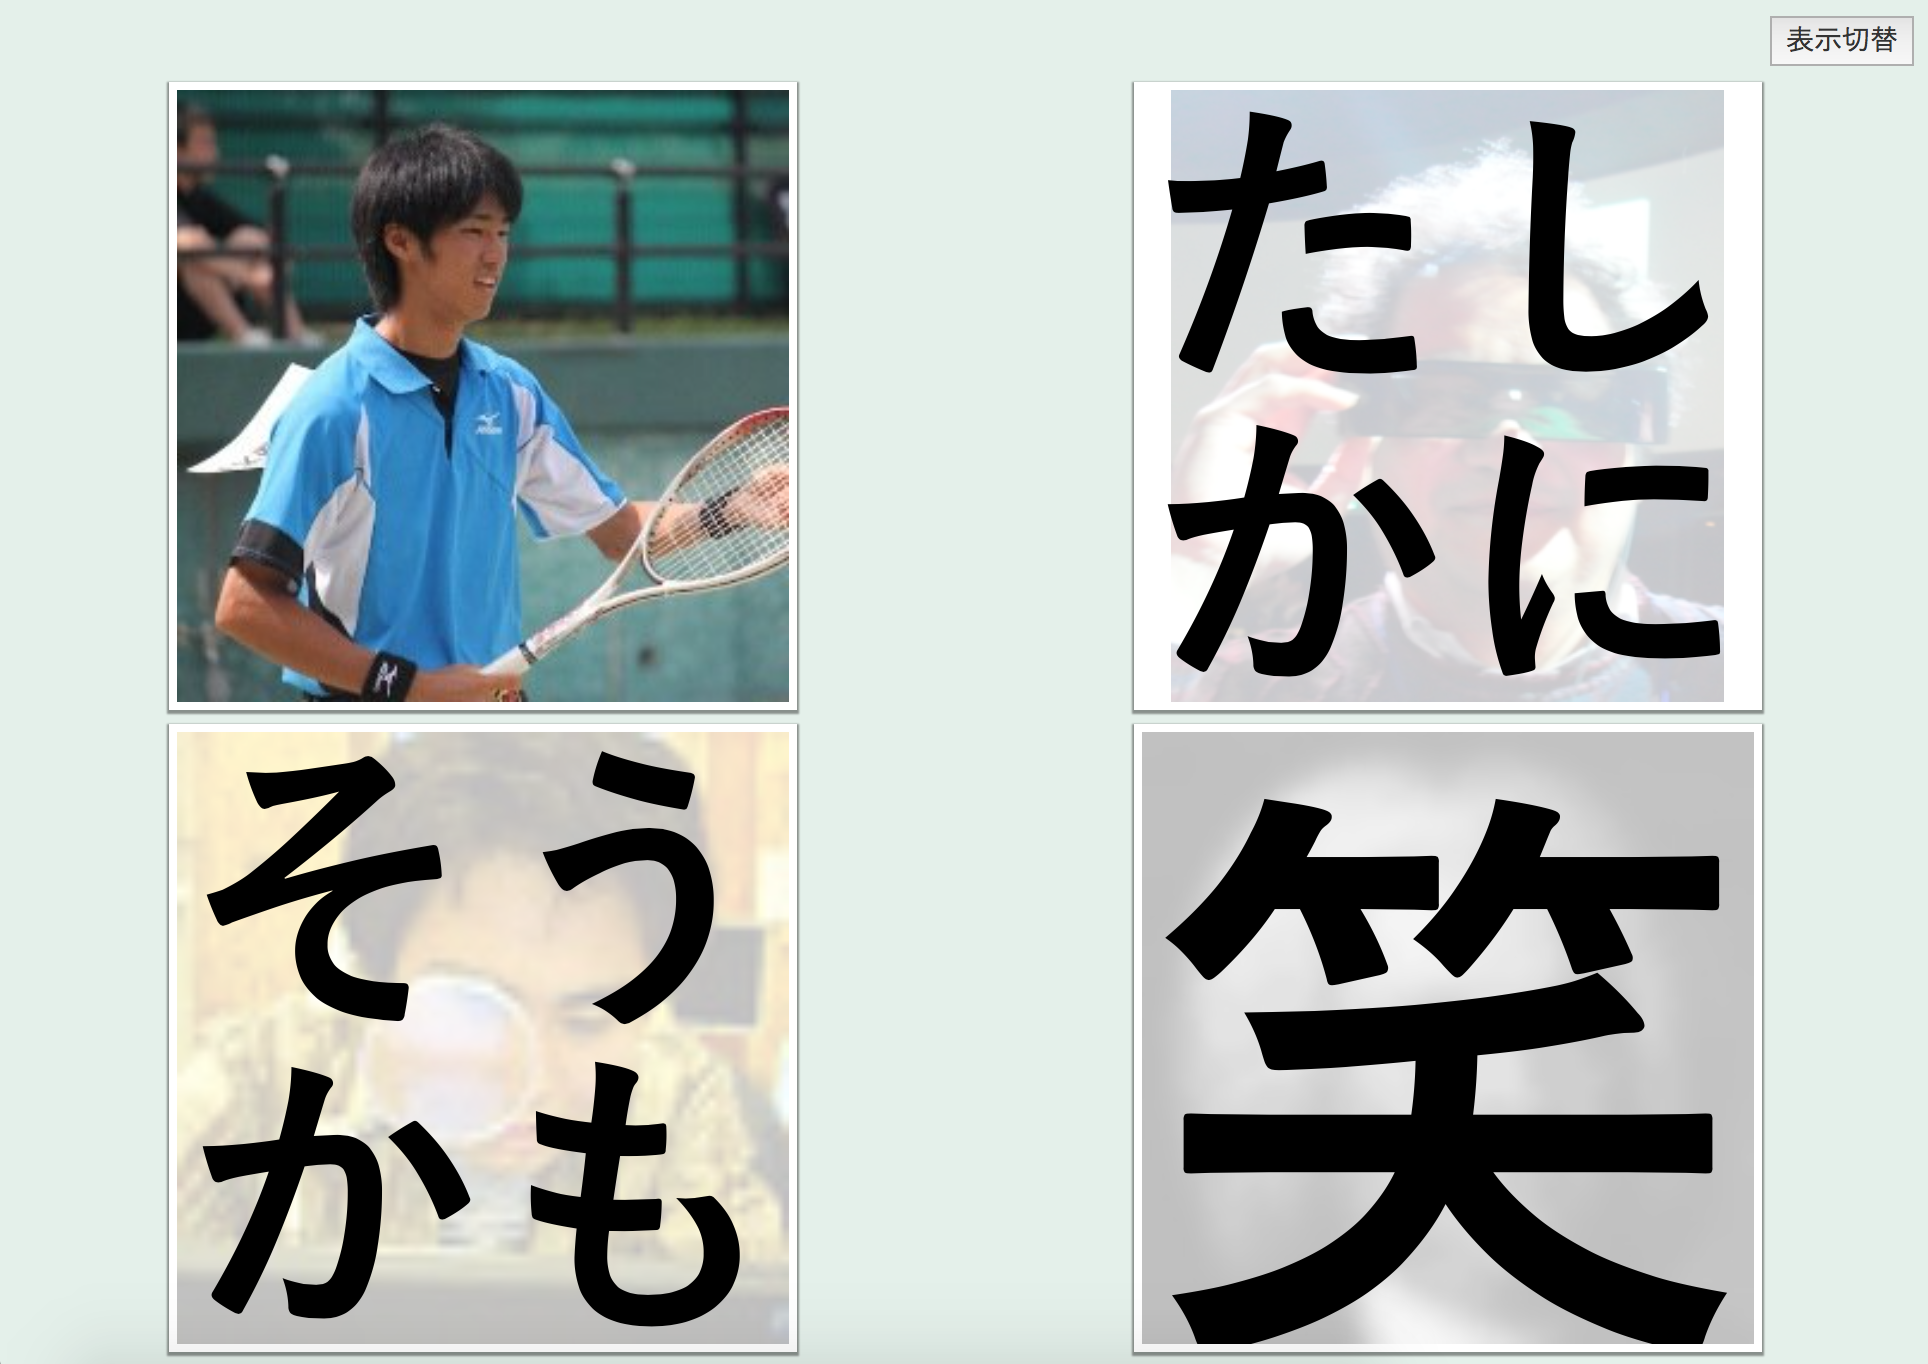
\includegraphics[width=7cm]{images/n_m_s_d.png}
\caption{4人のユーザを表示}
\label{n_m_s_d}
\end{figure}

\url{https://wakaruland.com/weather,temperature,wind}のように「\url{@}」を付けなかった場合は図\ref{w_t_w}のように\url{weather,temperature,wind}の3つがデータのセルとして表示される。

\begin{figure}[h]
\centering
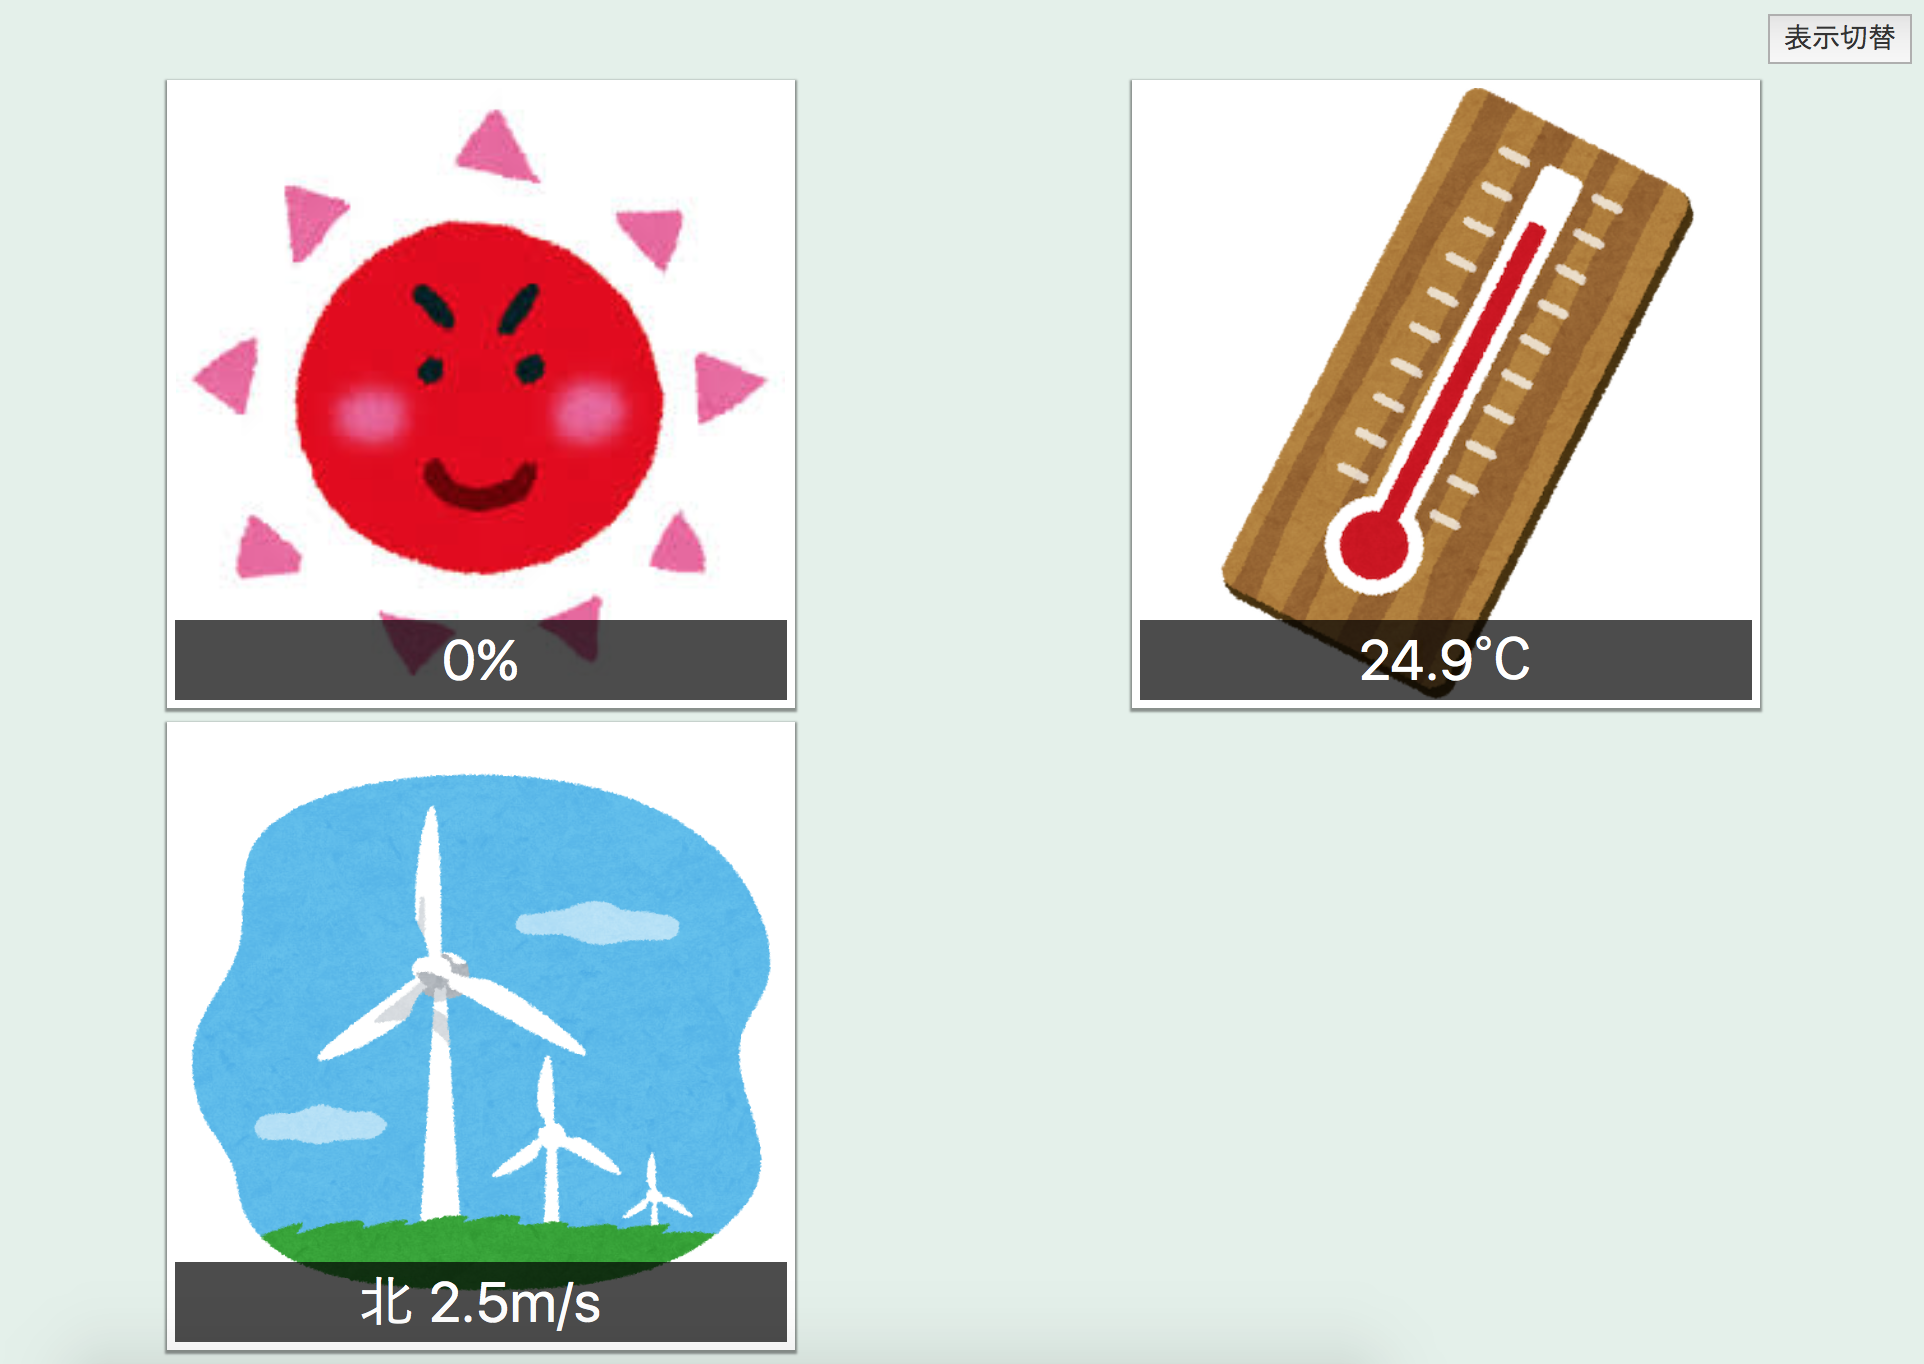
\includegraphics[width=7cm]{images/w_t_w.png}
\caption{3つのデータを表示}
\label{w_t_w}
\end{figure}

また、\url{https://wakaruland.com/@napo0703,weather,@masui,wind,@shokai}のようにリアクションとデータを合わせて表示させることも可能である(図\ref{n_w_m_w_s})。

\begin{figure}[h]
\centering
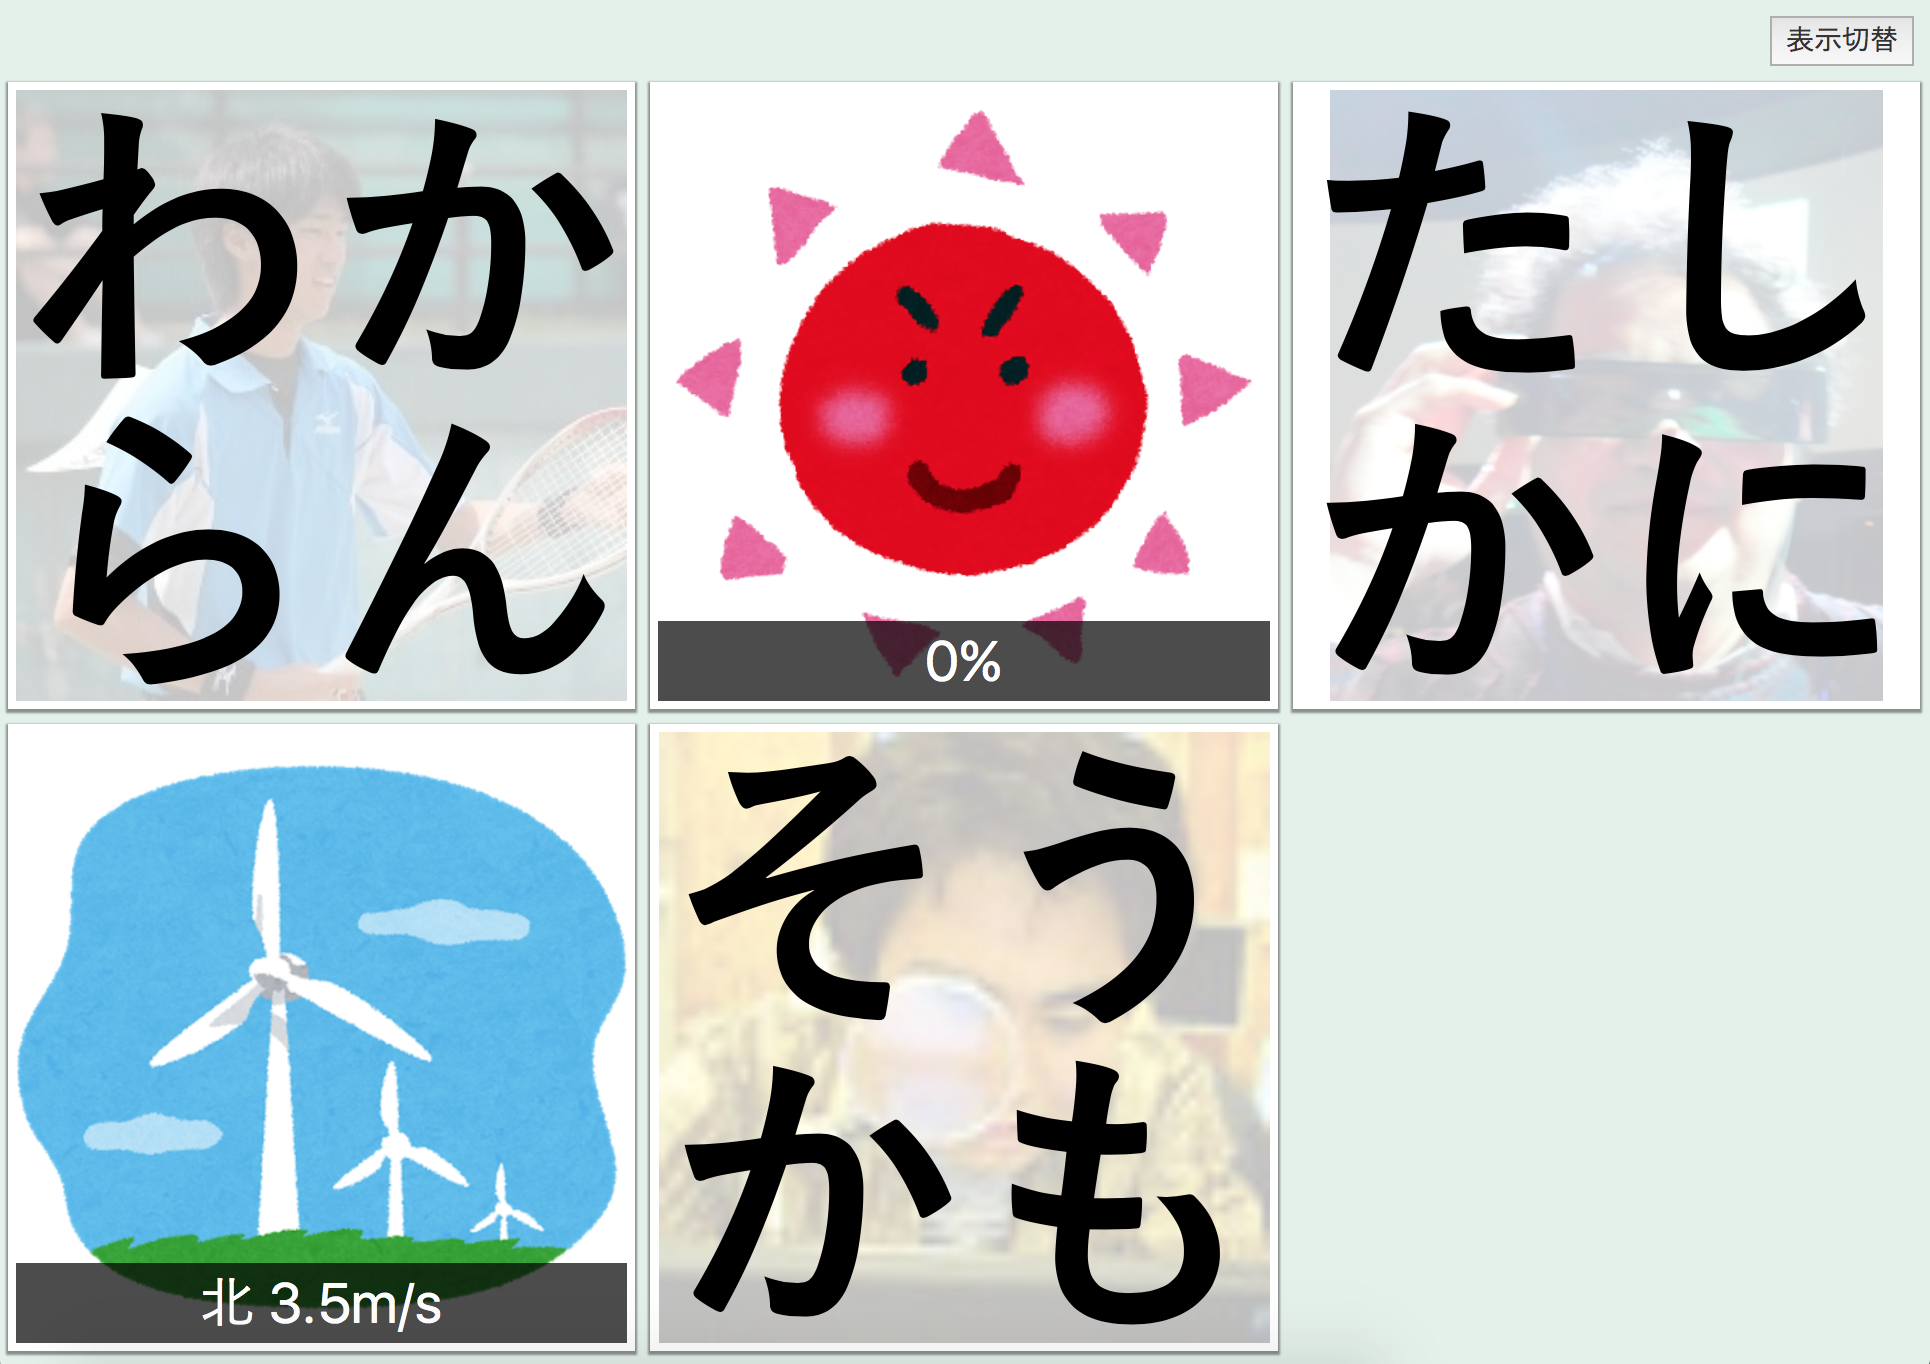
\includegraphics[width=7cm]{images/n_w_m_w_s.png}
\caption{ユーザとデータを表示}
\label{n_w_m_w_s}
\end{figure}

\subsection{スタンプの作成}
ユーザが投稿画面でリアクションとして投稿するスタンプには、
「画像」スタンプと「テキスト」スタンプの2種類がある(図\ref{stamp})。
ユーザは投稿画面のテキストボックスに文字列を入力し追加ボタンを押すことで新たにスタンプを作成して追加することができる。

画像スタンプは、テキストボックスに\url{http://masuilab.org/image.jpg}のようなWebにある
画像のURLを入力し追加ボタンを押すことで、URLの画像をスタンプとして一覧に追加することができる。
ローカルにある画像ファイルをスタンプとして追加したい場合は、Gyazoなどのアプリケーションを使って
WebにアップロードしURLを得ることで追加が可能である。

テキストスタンプは、テキストボックスにURLでないを文字列を入力し追加ボタンを押すことで作成できる。
図\ref{wakaran}左は「わからん」とテキストボックスに入力してスタンプを作成したものである。
この「わからん」は1行に表示されているが、「わか らん」と改行を入れたい場所に半角スペースを入力
することで、図\ref{wakaran}右のように2行で表示される。

スタンプの削除は、スタンプにマウスオーバーすると右上に表示される「×」ボタンを押すことで削除できる。

\begin{figure}[h]
\centering

\includegraphics[width=7cm]{images/stamp.png}
\caption{テキストスタンプ(左)と画像スタンプ(右)}
\label{stamp}
\end{figure}

\begin{figure}[h]
\centering

\includegraphics[width=7cm]{images/wakaran.png}
\caption{「わからん」スタンプ(左)と「わか らん」スタンプ(右)}
\label{wakaran}
\end{figure}

\subsection{利用例}
図\ref{discussion}は会議や発表の場での利用例である。これは誰かが何か変なことを言ったのに対してユーザが反応している様子である。

図\ref{sensors}はダッシュボードとしての利用例で、各種のセンサの値やWebの情報等を表示している。データはリアルタイムに最新のものに更新されていく。

\begin{figure}[h]
\centering
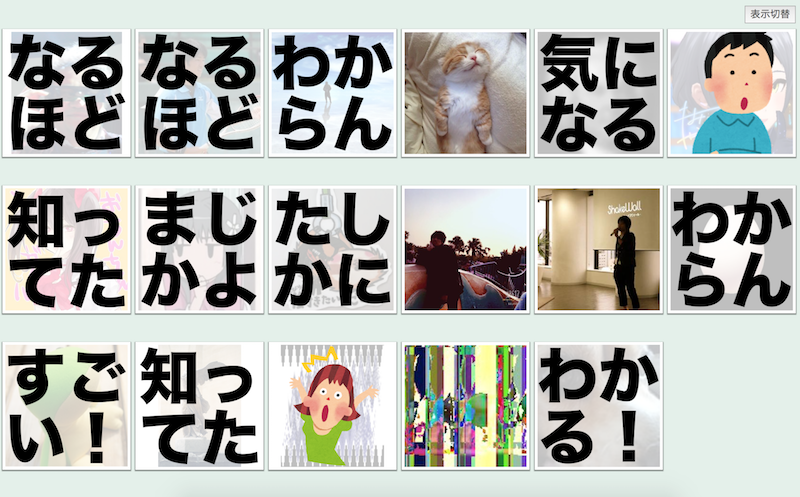
\includegraphics[width=7cm]{images/discussion.png}
\caption{会議や発表の場での利用例}
\label{discussion}
\end{figure}

\begin{figure}[h]
\centering
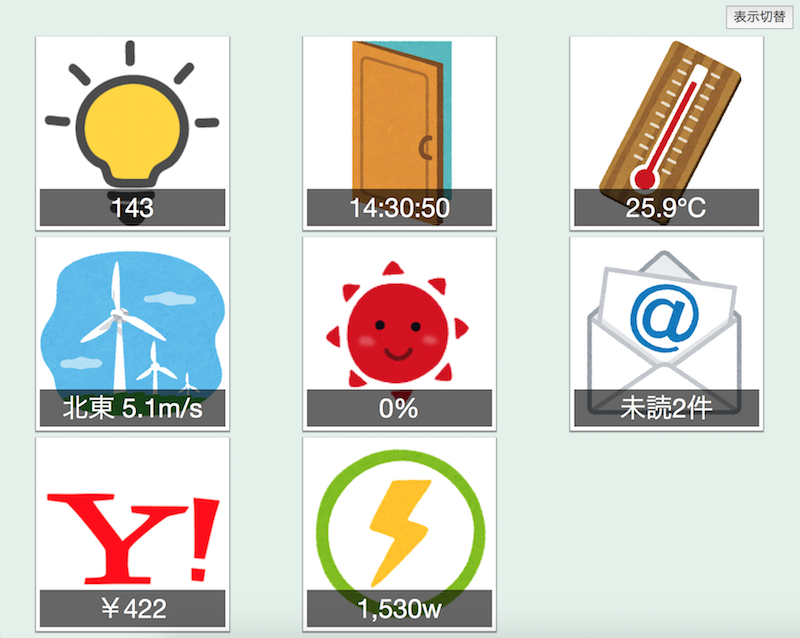
\includegraphics[width=7cm]{images/sensors.png}
\caption{ダッシュボードとしての利用例}
\label{sensors}
\end{figure}
\section{実装}

わかるらんどのクライアントは
HTML/CSS/JavaScriptで実装されており、
通常のブラウザ上のWebアプリケーションとして動作する。
%
サーバは、
並列計算プリミティブである
\textit{Linda}\cite{Carriero:1989:LC:63334.63337}を
Webサーバ上に実装した
WebLinda\footnote{https://github.com/node-linda/linda}を用いて実装している。

\subsection{Linda}

Lindaは、
複数のプロセスで共有される空間を用いて
プロセス間通信やデータ共有をサポートする
分散並列処理を行うためのモデルである。
プロセスが共有する空間は\textbf{タプル空間} (Tuple Space) と呼ばれ、
タプル空間内のデータ (Tuple) を使って通信やデータ共有を行う (図\ref{linda})。
Lindaのモデルはきわめて単純であるが、
各クライアントやデバイス間で直接送信をする処理を記述する必要がなく,
柔軟で強力なプロセス間通信を容易に記述することができる。

\begin{figure}[h]
\centering
\fbox{
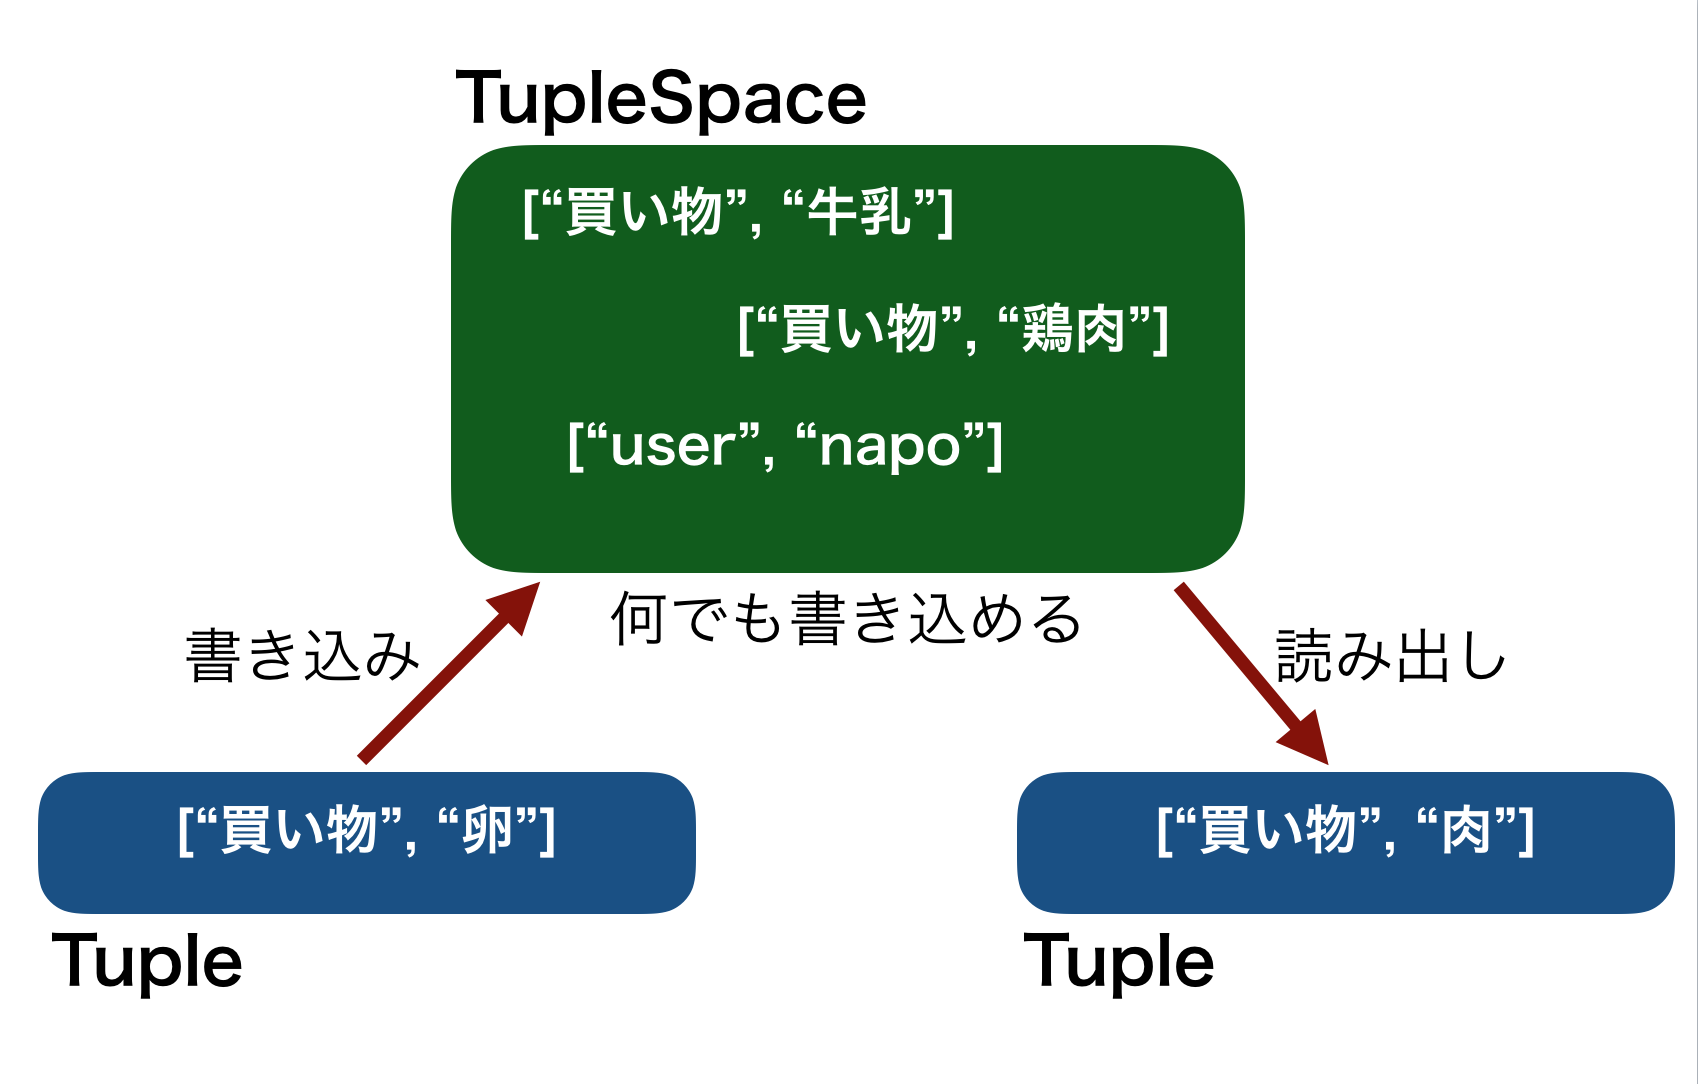
\includegraphics[width=7cm]{images/linda.png}
}
\caption{タプル空間を利用したプロセス間通信}
\label{button}
\end{figure}

\subsection{WebLinda}

WebLindaは、橋本翔氏が開発したオープンソースソフトウェアで、
% \footnote{http://shokai.org}
Node.js\footnote{https://nodejs.org}の
WebSocketライブラリ「Socket.IO\footnote{http://socket.io}」で
実装されている。
WebLindaは通常のWebサーバ上に実装されているため、
HTTP通信をサポートする様々な環境やプログラミング言語で利用可能である。

WebLindaは、\texttt{write}, \texttt{read}, \texttt{take}, \texttt{watch}という
4つの基本操作によってプロセス間通信を行う。

% ここは\enumerate じゃないのか?

\vspace{2mm}
\paragraph*{\texttt{write}}
新しいデータオブジェクト(タプル)を生成し共有空間(タプルスペース)に書き込む。

\vspace{4mm}
\paragraph*{\texttt{read}}
指定した形式に部分一致するタプルがタプルスペースにあるかどうか調べて1つ読み出す。
一致するものが無い場合は一致するタプルが書き込まれるまで待つ。

\vspace{2mm}
\paragraph*{\texttt{take}}
\texttt{read}しつつ、読み出したタプルをタプルスペースから削除する。

\vspace{2mm}
\paragraph*{\texttt{watch}}
タプルスペースを監視し、一致するタプルが
\texttt{write}された瞬間に読み出す。

\subsection{『わかるらんど』でのWebLinda実装}
『わかるらんど』でのWebLinda実装について述べる。
ユーザのリアクションを投稿/表示する際には、

\begin{lstlisting}
{
    type: "reaction",
    from: "@napo0703",
    display: "60",
    value: "なる ほど"
}
\end{lstlisting}
というようなタプルをやりとりしている。

センサやWebのデータを投稿/表示する際には、
\begin{lstlisting}
{
    type: "data",
    from: "明るさ",
    display: "60",
    value: "500",
    background: "http://masuilab.org/image.jpg"
}
\end{lstlisting}
というようなタプルをやりとりしている。

\vspace{4mm}
\paragraph*{type}
ユーザのリアクションの場合は\texttt{reaction}、
データの場合は\texttt{data}を値にする。

\vspace{4mm}
\paragraph*{from}
投稿元を表す値。

\vspace{2mm}
\paragraph*{display}
リアクションやデータの表示時間。単位は秒。リアクションやデータが表示されてからこの秒数が経過すると、自動的に取り下げられ表示されなくなる。20〜86400の間で指定が可能。

\vspace{2mm}
\paragraph*{value}
リアクションの場合、この値がWebにある画像ファイルのURLだった時は、その画像を投稿者のセルにオーバーレイ表示する。URLでない文字列の場合は、その文字列を投稿者のセルにオーバーレイ表示する。
データの場合、この値がそのままセルの下部に表示される。

\vspace{4mm}
\paragraph*{background}(データのみ)
データセルの背景画像のURL。そのデータが何を表すものなのか分かる画像を表示する。

\vspace{2mm}
以下は、ボタンを押した際に『わかるらんど』にユーザ「@napo0703」として「なる ほど」という「リアクション」を「20秒」表示するタプルを書き込むJavaScriptプログラムの例である。

\vspace{2mm}
\begin{lstlisting}
// Lindaに接続
const url = "http://linda.masuilab.org";
const socket = SocketIO(url);
const linda = new Linda().connect(socket);
const ts = linda.tuplespace("masuilab");

// ボタンを押したらタプルスペースにデータ書き込み
const button = $("button").click(function () {
  ts.write({
    type: "reaction",
    from: "@napo0703",
    display: "20",
    value: "http://masuilab.org/image.jpg",
  };
});
\end{lstlisting}

以下は、先程のプログラムで書き込まれるタプルと合致する
\texttt{{from: "@napo0703", type: "reaction"}}を含むタプルが書き込まれた場合に
リアクションを表示するJavaScriptプログラムの例である。

\vspace{2mm}
\begin{lstlisting}
// Lindaに接続
const url = "http://linda.masuilab.org";
const socket = SocketIO(url);
const linda = new Linda().connect(socket);
const ts = linda.tuplespace("masuilab");

// 合致するタプルが書き込まれたら画像を変える
ts.watch({
    from: "@napo0703",
    type: "reaction"
    }, function (tuple) {
  $("img").attr("src", tuple.data.value);
};
\end{lstlisting}

以下は現在の江ノ島の風向と風速をタプルスペースに書き込むRubyプログラムである。
NokogiriというライブラリでWebページから必要な情報をスクレイピングして
タプルスペースに書き込んでいる。

\vspace{2mm}
\begin{lstlisting}
url = 'http://linda.masuilab.org'
linda = Linda::SocketIO::Client.connect url
ts = linda.tuplespace('masuilab')

ts.on :connect do
  // Nokogiriでスクレイピング
  web = 'http://www.s-n-p.jp/kishou.htm'
  doc = Nokogiri::HTML(open(web))
  // 必要な情報を取得
  tds = doc.xpath("//td")
  as = tds[16].xpath(".//b").text.sub(/[^\d\.].*$/,'')
  ad = tds[19].xpath(“.//b”).text
  // タプルスペースに書き込み
  ts.write(
      where: 'enoshima',
      type: 'data',
      name: 'wind',
      value: ad + as.to_f + ‘m/s')
end
\end{lstlisting}
\section{議論}

\subsection{『わかるらんど』の思想}

近年、学会などでタイムライン表示のテキストチャットが利用されることが
多くなっている\cite{WISSのチャットの報告論文}。
発表中に参加者が意見交換したり疑問を表明したりできるので、
学会チャットシステムは大変有用なものであるが、
以下のような問題も存在する。

\begin{itemize}
\item 同時に多数が投稿するとすぐに流れていってしまう
\item 投稿数の多い人ばかりが目立ってしまう
\item 投稿しない人は全く投稿しない
\end{itemize}

世の中の会議において、
特定の人だけが沢山発言するのはよくあることであるが、
誰もが気軽に意見を表明できる環境を構築できれば有意義であろう。

「On Air Forum」は、日本ソフトウェア科学会主催のWISSで利用されている
コミュニケーションシステムである。
「On Air Forum」のWISS2009の実証実験\cite{nishida2011}では、
全参加者の半分弱しかログインして1回以上発言していない.
WISS2015では、252アカウントが1回以上発言し総発言数は2,948回であったが、
発言数上位20\%の50アカウントによる発言が総発言数の78.1\%にあたる2,305回を占めていた(図\ref{wisschat})。
また、発言数が10回未満のアカウントは190アカウントで、これは全アカウントの75.3\%にあたる。

\begin{figure}[h]
\centering
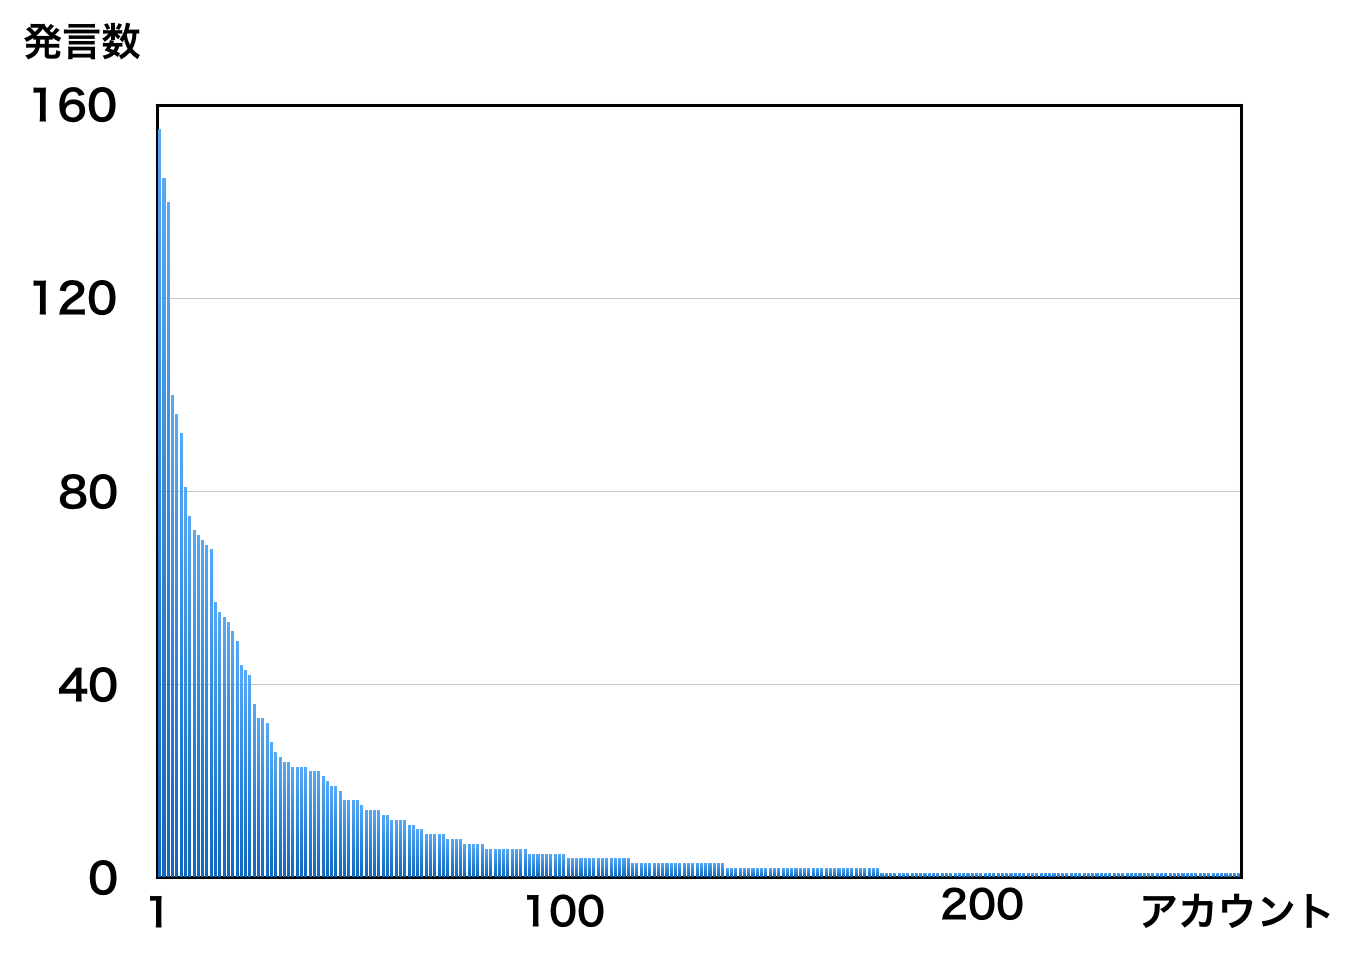
\includegraphics[width=7cm]{images/wisschat.png}
\caption{WISS2016のチャットにおけるアカウント毎の発言数}
\label{wisschat}
\end{figure}

『わかるらんど』はユーザの表示領域が均等に決まっているため、
タイムライン表示のように投稿数が多い人ばかりが目立つということがない。
また、長いテキストを入力すると表示される文字が小さくなるので、
150人程度で利用すると長い文字は小さすぎて読めない。
必然的にユーザは図\ref{wakaruland150}のように短文を入力することを強いられる。
『わかるらんど』では長文の高度な発言は期待しておらず、
「なるほど」「わからん」「笑」などといった相槌のようなものを
視覚化してひと目で把握できるようになることを期待している。
学生、先生、企業に所属する人等様々なバックグラウンドの人が入り混じった状況で
「下手な発言ができない」「気の利いたことを言わなければならない」という
投稿を躊躇させる要素を限りなく減らし、
本当は議論に参加したいけど声が出ない/手を上げる勇気がない人でも
「なるほど」「わかる」などを『わかるらんど』に投稿することで「参加」することができる。
テキストで記述すると長くなってしまう内容も
画像スタンプを投稿することで分かってもらうことができると考える。
また、長いテキストを投稿するには適していないので『わかるらんど』を使って議論することは難しいが、
多くの会議やコンファレンスでは発表後に議論の時間が設けられているため議論はその時に行えばよい。

\begin{figure}[h]
\centering
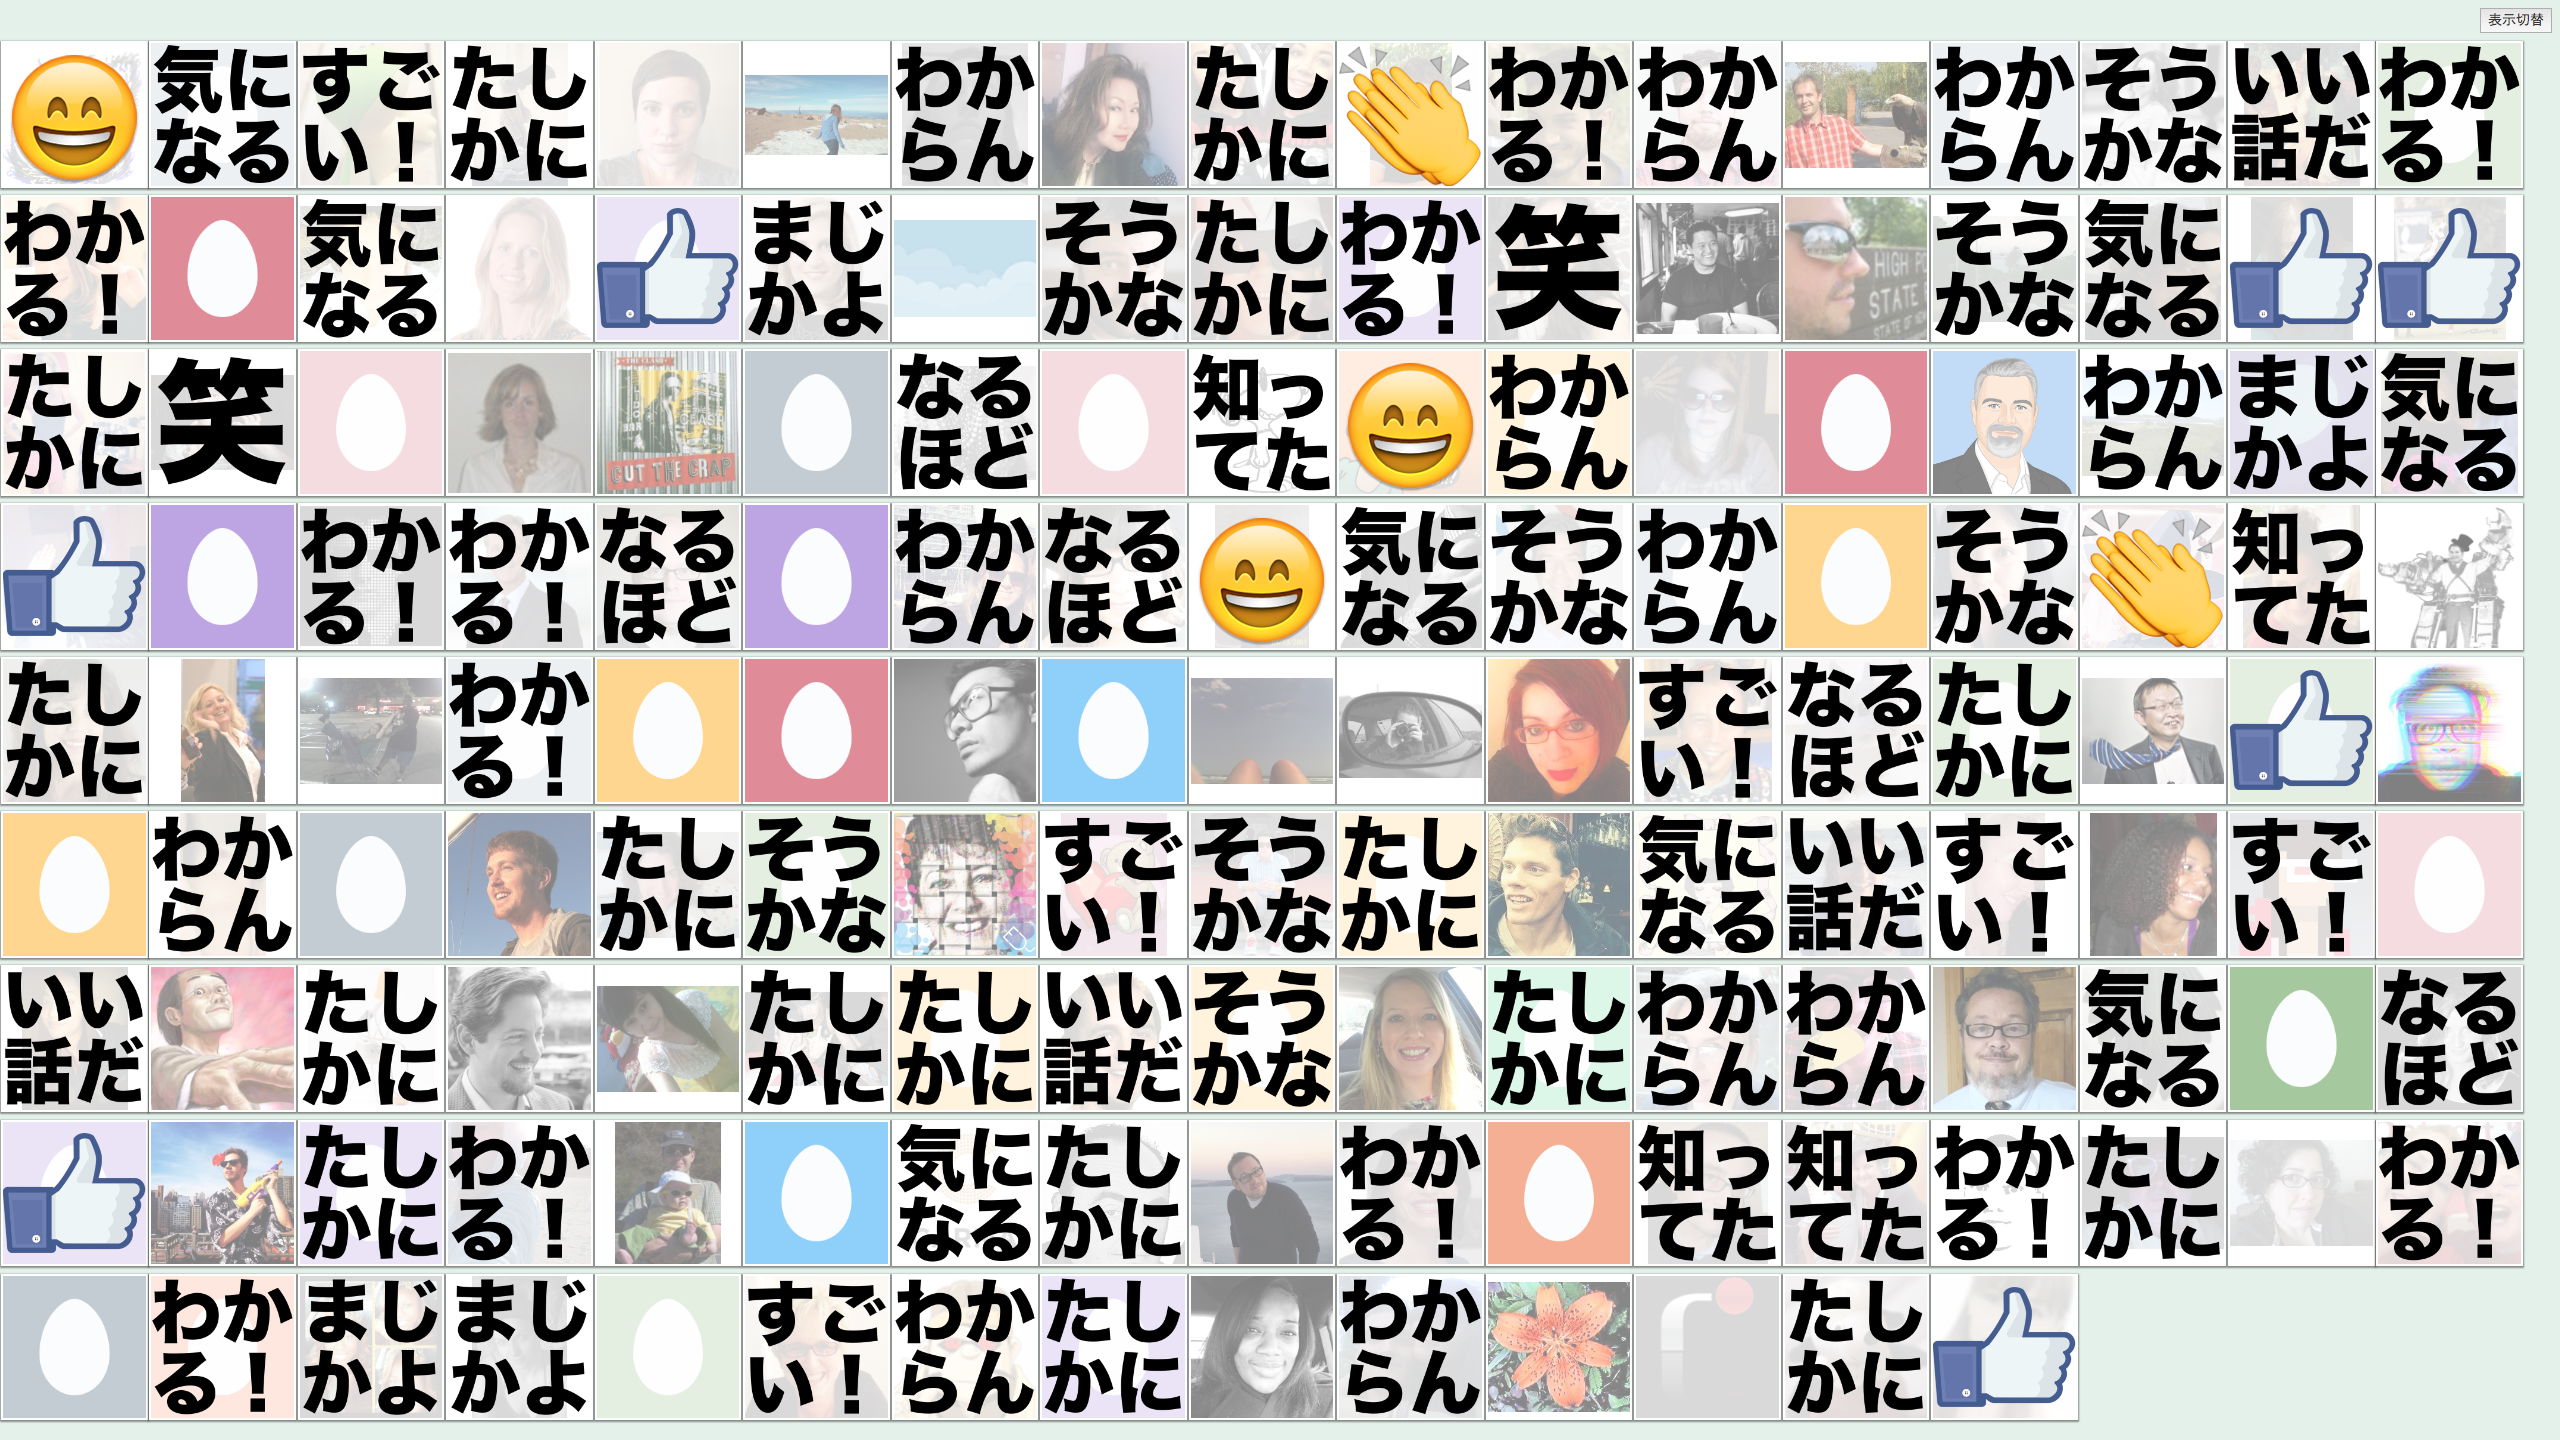
\includegraphics[width=8cm]{images/wakaruland150.png}
\caption{150人で『わかるらんど』を使用したイメージ}
\label{wakaruland150}
\end{figure}

\subsection{研究室においての利用経験}
我々の研究室では、研究室内のディスプレイに研究室メンバー全員のリアクションと
部屋の明るさ、温度、最後に研究室のドアが開いた時間を表示した『わかるらんど』を
常に表示して、約6ヶ月の間利用してきた。
ミーティングの時間には積極的に『わかるらんど』を利用した。
普段発言の少ない人でも何らかの反応を表明したり、
誰かが面白いことを言ったときに「笑」というリアクションが並ぶと面白かった。
また発表者としても、聴衆が自分の発表を聞いてくれているかどうかわからないときに
『わかるらんど』にリアクションを投稿してもらうことで、聴衆がみんなPCの画面を見ていても
何らかの投稿があれば話を聞いているということがわかるようになった。
自分が研究室にいないときでもリアクションを投稿して、
研究室でも自宅でも研究室メンバーの気分や研究室のセンサ情報が見られるようになった。

研究室で利用しているチャットでチャットボットに話しかけることで、研究室の
\begin{itemize}
  \item ドアの鍵を開ける
  \item 照明を点ける/消す
  \item 明るさを知る
  \item 気温を知る
\end{itemize}
ことができるが、『わかるらんど』と組み合わせることで非常に便利に使うことができた。



\section{関連研究}
関連する研究には,
\begin{itemize}
\item 情報ダッシュボード
\item 多くの人がいる場での計算機を用いたコミュニケーション
\end{itemize}
に関するものがある

\subsection{情報ダッシュボードに関する研究}
研究としては,2つに区切られたレイアウトのダッシュボードのセルの配置を支援するもの
\cite{Hertzog:2015:BSP:2678025.2701383}や,
ある課題の解決のためにどのような情報をダッシュボードに表示するべきか
\cite{Jones:2015:ECI:2800835.2800963}などが議論されている.
ダッシュボードに人間の感情や現在の状況を表示するといった研究は今までに行われていない.

\subsection{多くの人がいる場での計算機を用いたコミュニケーションの研究}
「Lock-on-Chat\cite{nishida2006}」は複数の話題に分散した会話を促進するチャットシステムである.
先に述べた「On Air Forum」はリアルタイムコンテンツを視聴中のコミュニケーションシステムである.

また,消極性研究会(SIGSHY: Special Interest Group on Shyness and Hesitation around You)という
グループが,消極的な人と積極的な人が混在する場のデザインとICT支援について研究しており,
大勢の人が集まる場で消極的な人でも誰かと交流することを支援するようなシステム\cite{nishida2011}が
研究されていたり,消極性研究に関する書籍\cite{kurihara2016}も出版されている.

\section{まとめ}
本論文では、実世界の状態や人間の状況を情報ダッシュボードにわかりやすく表示し、
かつ誰もが簡単に気分などをスタンプのように投稿して共有できる「わかるらんど」システムを提案した。


\bibliographystyle{ipsjsort}
\bibliography{paper}

\end{document}
